\section{Discussion and Conclusion}  \label{sec:Conclu}
%Comparing with the state of the art SDN frameworks in \cite{IF14iSTAMP:2014} and \cite{Adrichen:2014} that have been used for \emph{fine-grained} network performance measurements, SNIPER can be used in a wide range of network monitoring applications under hard network resource constraints while, it is still capable of providing estimates of IAI with acceptable accuracy and reliability, based on the application. The computational complexity and communication overhead of the SNIPER frame work are low while it does not suffer from feasibility constraints as in \cite{IF14iSTAMP:2014}. Such capabilities are based on the fact that: 1) the SNIPER is a SDN measurement framework; 2) the main NI technique in SNIPER is the matrix completion algorithm, where providing the required measurement of IAI is feasible, and 3) the OOM required by matrix completion techniques is designed using EOAs to provide the most informative measurements with the smallest amount of resources. We showed that SNIPER is a generic, flexible and efficient framework that can be used for a variety of network monitoring applications under hard resource constraints.
Table \ref{tab:SDNFrmCmp} compares the performance of SNIPER with the state of the art SDN frameworks in \cite{IF14iSTAMP:2014} and \cite{Adrichen:2014} that have been used for \emph{fine-grained} network performance measurements. The comparison in this table is qualitative because the exact comparison between SNIPER and these two frameworks is difficult due to the facts that: 1) the traffic matrix estimation techniques and criterion in \cite{IF14iSTAMP:2014} are different from SNIPER, and 2) in \cite{Adrichen:2014}, the IAI are directly measured for different network(s) where the same data-sets are unavailable.

This table shows that there is a tradeoff between different parameters that must be considered in the design of effective network measurement systems. Among these, SNIPER can be used in a wide range of network monitoring applications under hard network resource constraints while, it is still capable of providing estimates of IAI with acceptable accuracy and reliability, based on the application. The computation and communication overhead of the SNIPER frame work are low while it does not suffer from feasibility constraints as in \cite{IF14iSTAMP:2014}. Such capabilities are based on the fact that: 1) the SNIPER is a SDN measurement framework with high flexibility; 2) the main NI technique in SNIPER is matrix completion algorithm, where providing the required independent measurements of IAI is feasible, and 3) the OOM required by MC techniques is designed using EOAs to provide the most informative measurements with the smallest amount of resources. We showed the effectiveness of SNIPER in different network monitoring applications and under hard resource constraints.

\begin{table}
\centering
	{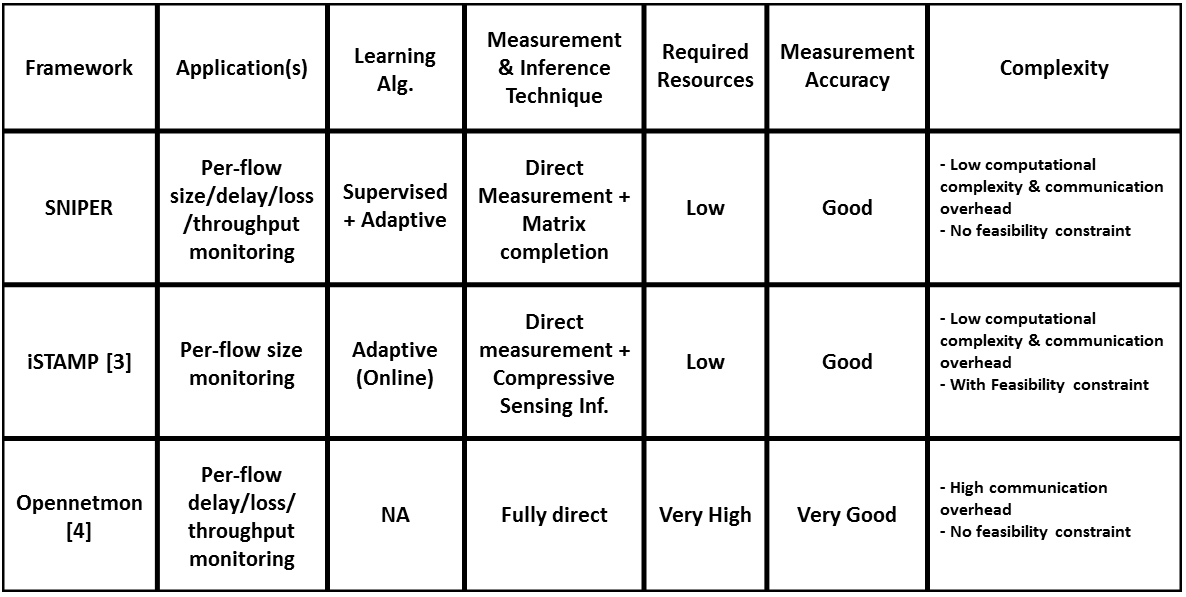
\includegraphics[keepaspectratio, width=0.42\textwidth]{CompTable_New2.png}} 
  % \includegraphics[width=\linewidth]{excel-table}
  \caption{{A comparison between SDN network measurement frameworks.}}
  \label{tab:SDNFrmCmp}
\end{table}


%In this paper we introduced SNIPER, an intelligent network measurement framework, where the flexibility provided by SDN is used to optimally design the observation or measurement matrix which leads to the best possible estimation accuracy via applying matrix completion techniques. 
%Since the design of optimal binary observation matrices using integer optimization techniques is extremely complicated and computationally expensive, here, we have formulated this problem using evolutionary optimization algorithms including genetic algorithm and particle swarm optimization algorithm. We have shown that both methods can be used by the SNIPER framework to effectively design the optimal measurement matrices under hard constraint of measurement resources. The effectiveness of this method have been examined using both synthetic and real network measurement traces from different network topologies and by considering two main applications including network traffic and delay estimations. The feasibility of our framework has also verified by implementing a prototype of SNIPER in Mininet environment.
%In this paper we introduced SNIPER, an intelligent network measurement framework, where the flexibility provided by SDN is used to optimally design the observation or measurement matrix which leads to the best possible estimation accuracy via applying matrix completion techniques. 
%Since the design of optimal binary observation matrices using integer optimization techniques is extremely complicated and computationally expensive, here, we have formulated this problem using evolutionary optimization algorithms including genetic algorithm and particle swarm optimization algorithm. We have shown that both methods can be used by the SNIPER framework to effectively design the optimal measurement matrices under hard constraint of measurement resources. The effectiveness of this method have been examined using both synthetic and real network measurement traces from different network topologies and by considering two main applications including network traffic and delay estimations. The feasibility of our framework has also verified by implementing a prototype of SNIPER in Mininet environment.
% SNIPER in recommended systems by intelligent and active interaction with the system to sample the best points


%\begin{table}
	%\centering
%%  \footnotesize{
 %\small{
 %% \renewcommand{\tabcolsep}{0.05cm}
 %% \renewcommand{\arraystretch}{1.0}
		%\begin{tabular}{| c | c | c | c | c | c | c | c |}
		%\hline
       %Framework &    \\ \hline
    %\end{tabular}
	%\caption{\scriptsize{The average of $P^{d}_{CP}$ and $P^{fa}_{CP}$ for Harvard network in different sampling ratios.}}
	%\label{tab:PdfaHarvard}
%}
%\end{table}
